\documentclass{standalone}
\usepackage{tikz}
\usetikzlibrary{patterns, positioning}
\usepackage[sfdefault]{ClearSans} %% option 'sfdefault' activates Clear Sans as the default text font
\usepackage[T1]{fontenc}

\begin{document}
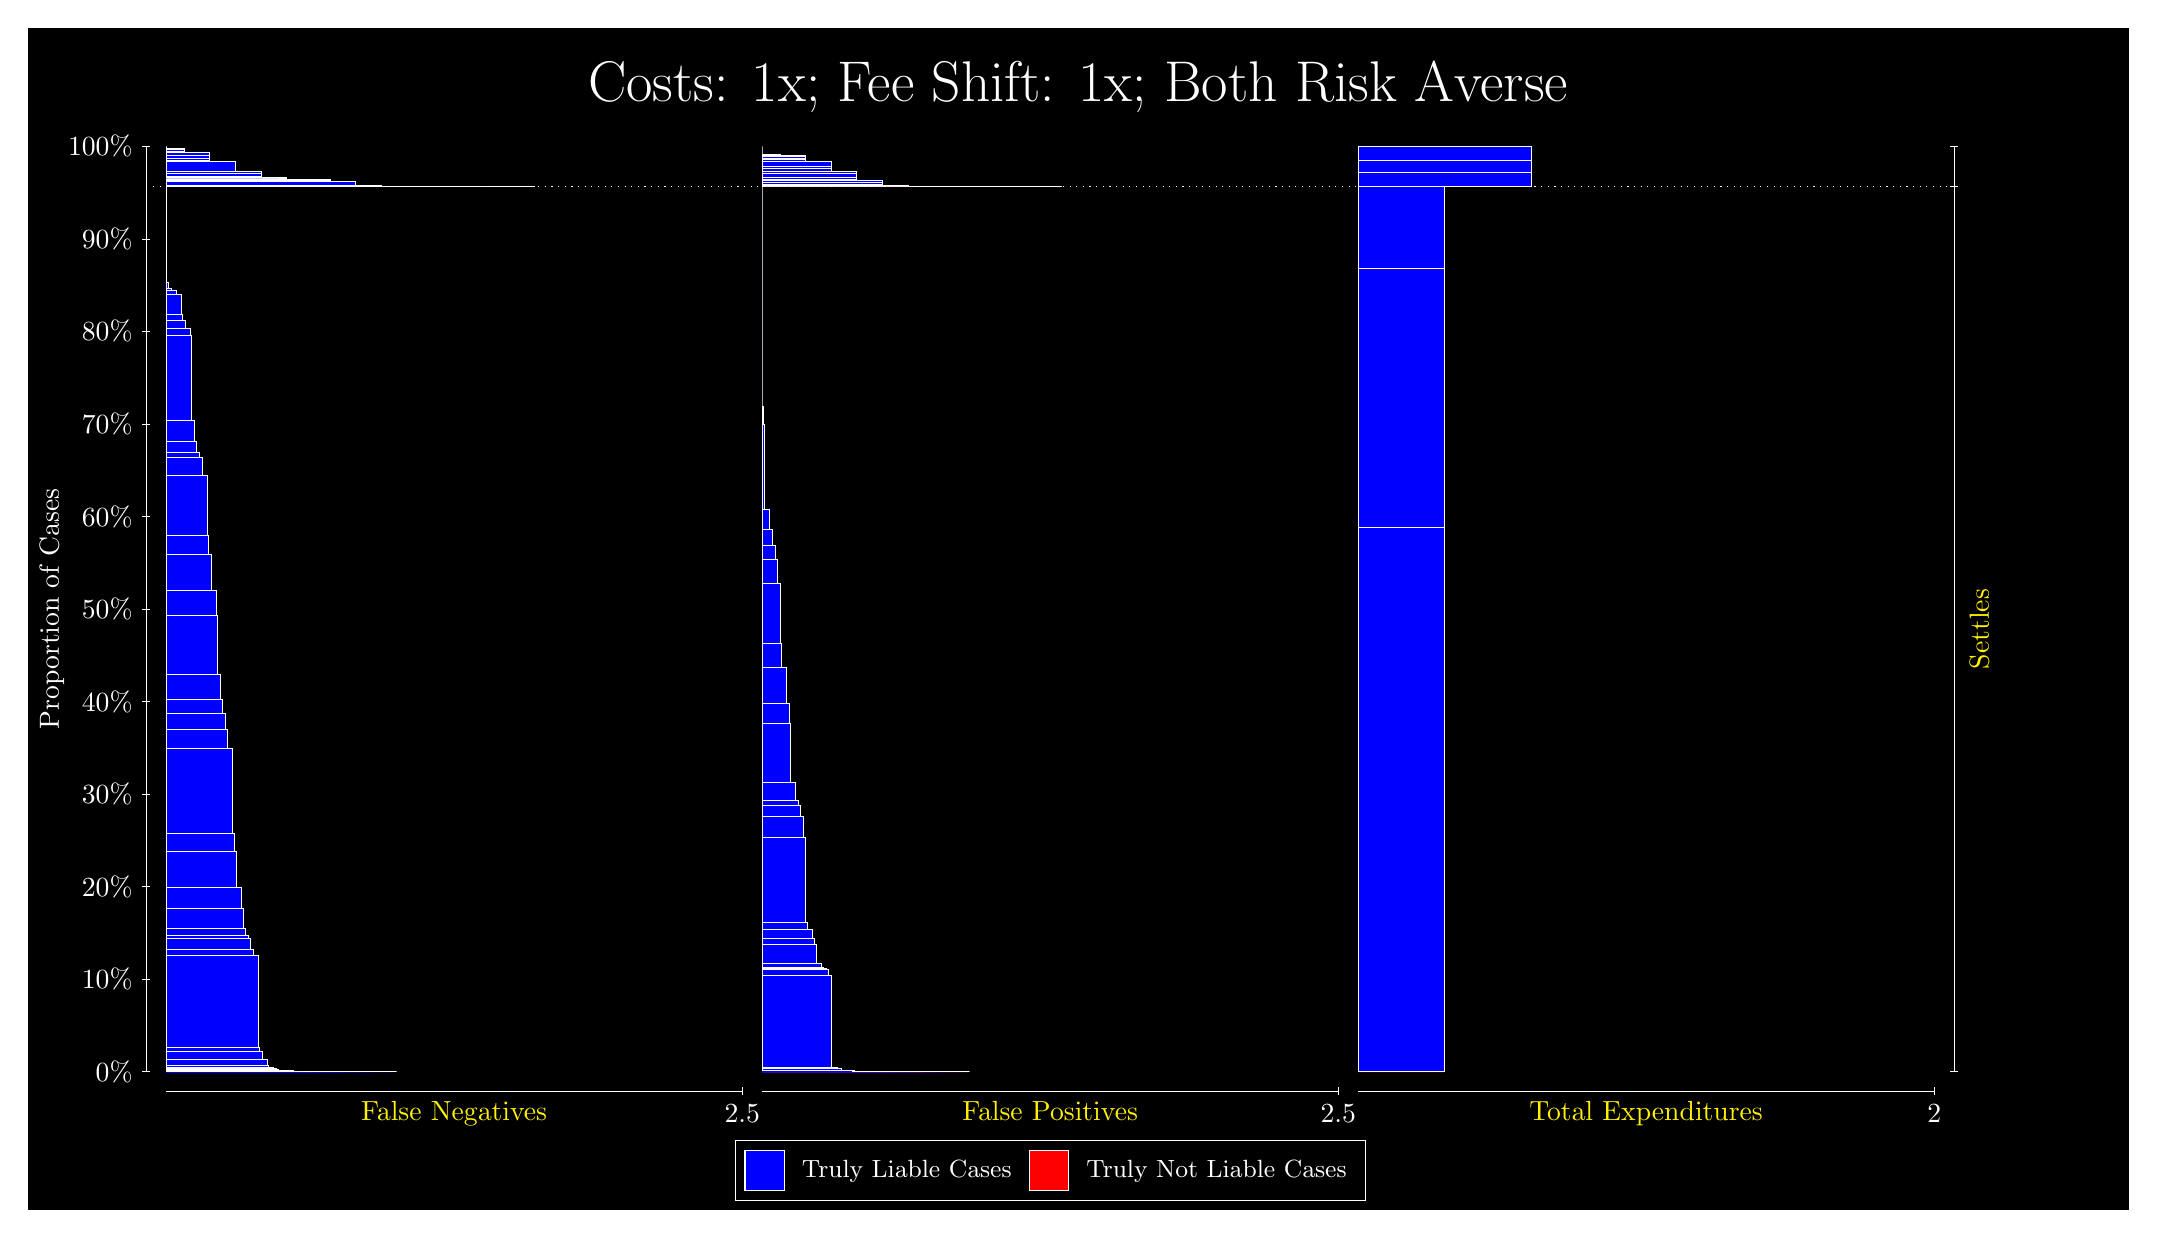
\begin{tikzpicture}
\draw[fill=black] (0,0) rectangle (26.667,15);
\draw[text=white] (0,13.5) rectangle (26.667,15) node[midway] {\huge Costs: 1x; Fee Shift: 1x; Both Risk Averse};
\draw[white, very thin] (1.5,1.75) -- (1.5,13.5);
\node[rotate=90, text=white, anchor=center] at (0.3, 7.625) {Proportion of Cases};
\draw[white, very thin] (1.45,1.75) -- (1.55,1.75);
\node[text=white, anchor=east] at (1.45, 1.75) {0\%};
\draw[white, very thin] (1.45,2.925) -- (1.55,2.925);
\node[text=white, anchor=east] at (1.45, 2.925) {10\%};
\draw[white, very thin] (1.45,4.1) -- (1.55,4.1);
\node[text=white, anchor=east] at (1.45, 4.1) {20\%};
\draw[white, very thin] (1.45,5.275) -- (1.55,5.275);
\node[text=white, anchor=east] at (1.45, 5.275) {30\%};
\draw[white, very thin] (1.45,6.45) -- (1.55,6.45);
\node[text=white, anchor=east] at (1.45, 6.45) {40\%};
\draw[white, very thin] (1.45,7.625) -- (1.55,7.625);
\node[text=white, anchor=east] at (1.45, 7.625) {50\%};
\draw[white, very thin] (1.45,8.8) -- (1.55,8.8);
\node[text=white, anchor=east] at (1.45, 8.8) {60\%};
\draw[white, very thin] (1.45,9.975) -- (1.55,9.975);
\node[text=white, anchor=east] at (1.45, 9.975) {70\%};
\draw[white, very thin] (1.45,11.15) -- (1.55,11.15);
\node[text=white, anchor=east] at (1.45, 11.15) {80\%};
\draw[white, very thin] (1.45,12.325) -- (1.55,12.325);
\node[text=white, anchor=east] at (1.45, 12.325) {90\%};
\draw[white, very thin] (1.45,13.5) -- (1.55,13.5);
\node[text=white, anchor=east] at (1.45, 13.5) {100\%};

\draw[white, very thin] (24.457,1.75) -- (24.457,13.5);
\draw[white, very thin] (24.407,1.75) -- (24.507,1.75);
\node[anchor=west] at (24.407, 1.75) {};
\draw[white, very thin] (24.407,12.991) -- (24.507,12.991);
\node[anchor=west] at (24.407, 12.991) {};
\draw[white, very thin] (24.407,13.5) -- (24.507,13.5);
\node[anchor=west] at (24.407, 13.5) {};

\draw[white, very thin, fill=blue] (1.75,1.75) rectangle (4.6775,1.75);
\draw[white, very thin, fill=blue] (1.75,1.75) rectangle (4.3848,1.75);
\draw[white, very thin, fill=blue] (1.75,1.75) rectangle (4.3523,1.75);
\draw[white, very thin, fill=blue] (1.75,1.75) rectangle (4.2384,1.75);
\draw[white, very thin, fill=blue] (1.75,1.75) rectangle (4.092,1.75);
\draw[white, very thin, fill=blue] (1.75,1.75) rectangle (4.0595,1.75);
\draw[white, very thin, fill=blue] (1.75,1.75) rectangle (4.027,1.75);
\draw[white, very thin, fill=blue] (1.75,1.75) rectangle (3.9457,1.75);
\draw[white, very thin, fill=blue] (1.75,1.75) rectangle (3.9131,1.75);
\draw[white, very thin, fill=blue] (1.75,1.75) rectangle (3.7993,1.75);
\draw[white, very thin, fill=blue] (1.75,1.75) rectangle (3.7668,1.75);
\draw[white, very thin, fill=blue] (1.75,1.75) rectangle (3.7342,1.75);
\draw[white, very thin, fill=blue] (1.75,1.75) rectangle (3.7017,1.75);
\draw[white, very thin, fill=blue] (1.75,1.75) rectangle (3.6204,1.7501);
\draw[white, very thin, fill=blue] (1.75,1.7501) rectangle (3.5878,1.7501);
\draw[white, very thin, fill=blue] (1.75,1.7501) rectangle (3.5065,1.7505);
\draw[white, very thin, fill=blue] (1.75,1.7505) rectangle (3.474,1.751);
\draw[white, very thin, fill=blue] (1.75,1.751) rectangle (3.4415,1.751);
\draw[white, very thin, fill=blue] (1.75,1.751) rectangle (3.4089,1.751);
\draw[white, very thin, fill=blue] (1.75,1.751) rectangle (3.3764,1.7515);
\draw[white, very thin, fill=blue] (1.75,1.7515) rectangle (3.3602,1.7617);
\draw[white, very thin, fill=blue] (1.75,1.7617) rectangle (3.2951,1.767);
\draw[white, very thin, fill=blue] (1.75,1.767) rectangle (3.2626,1.7692);
\draw[white, very thin, fill=blue] (1.75,1.7692) rectangle (3.1812,1.7769);
\draw[white, very thin, fill=blue] (1.75,1.7769) rectangle (3.1487,1.7963);
\draw[white, very thin, fill=blue] (1.75,1.7963) rectangle (3.1162,1.7985);
\draw[white, very thin, fill=blue] (1.75,1.7985) rectangle (3.0837,1.8032);
\draw[white, very thin, fill=blue] (1.75,1.8032) rectangle (3.0511,1.8274);
\draw[white, very thin, fill=blue] (1.75,1.8274) rectangle (3.0349,1.9032);
\draw[white, very thin, fill=blue] (1.75,1.9032) rectangle (2.9698,2.0107);
\draw[white, very thin, fill=blue] (1.75,2.0107) rectangle (2.9373,2.0597);
\draw[white, very thin, fill=blue] (1.75,2.0597) rectangle (2.921,3.2238);
\draw[white, very thin, fill=blue] (1.75,3.2238) rectangle (2.856,3.2972);
\draw[white, very thin, fill=blue] (1.75,3.2972) rectangle (2.8234,3.4383);
\draw[white, very thin, fill=blue] (1.75,3.4383) rectangle (2.7909,3.4828);
\draw[white, very thin, fill=blue] (1.75,3.4828) rectangle (2.7584,3.5705);
\draw[white, very thin, fill=blue] (1.75,3.5705) rectangle (2.7258,3.821);
\draw[white, very thin, fill=blue] (1.75,3.821) rectangle (2.7096,4.0876);
\draw[white, very thin, fill=blue] (1.75,4.0876) rectangle (2.6445,4.5461);
\draw[white, very thin, fill=blue] (1.75,4.5461) rectangle (2.612,4.7725);
\draw[white, very thin, fill=blue] (1.75,4.7725) rectangle (2.5957,5.8562);
\draw[white, very thin, fill=blue] (1.75,5.8562) rectangle (2.5307,6.1018);
\draw[white, very thin, fill=blue] (1.75,6.1018) rectangle (2.4982,6.3035);
\draw[white, very thin, fill=blue] (1.75,6.3035) rectangle (2.4656,6.4809);
\draw[white, very thin, fill=blue] (1.75,6.4809) rectangle (2.4331,6.792);
\draw[white, very thin, fill=blue] (1.75,6.792) rectangle (2.4006,7.5478);
\draw[white, very thin, fill=blue] (1.75,7.5478) rectangle (2.3843,7.8589);
\draw[white, very thin, fill=blue] (1.75,7.8589) rectangle (2.3192,8.3174);
\draw[white, very thin, fill=blue] (1.75,8.3174) rectangle (2.2867,8.5631);
\draw[white, very thin, fill=blue] (1.75,8.5631) rectangle (2.2705,9.3188);
\draw[white, very thin, fill=blue] (1.75,9.3188) rectangle (2.2054,9.5453);
\draw[white, very thin, fill=blue] (1.75,9.5453) rectangle (2.1729,9.614);
\draw[white, very thin, fill=blue] (1.75,9.614) rectangle (2.1403,9.7501);
\draw[white, very thin, fill=blue] (1.75,9.7501) rectangle (2.1078,10.017);
\draw[white, very thin, fill=blue] (1.75,10.017) rectangle (2.0753,11.1);
\draw[white, very thin, fill=blue] (1.75,11.1) rectangle (2.059,11.188);
\draw[white, very thin, fill=blue] (1.75,11.188) rectangle (1.994,11.295);
\draw[white, very thin, fill=blue] (1.75,11.295) rectangle (1.9614,11.369);
\draw[white, very thin, fill=blue] (1.75,11.369) rectangle (1.9452,11.619);
\draw[white, very thin, fill=blue] (1.75,11.619) rectangle (1.8801,11.668);
\draw[white, very thin, fill=blue] (1.75,11.668) rectangle (1.8476,11.676);
\draw[white, very thin, fill=blue] (1.75,11.676) rectangle (1.8151,11.695);
\draw[white, very thin, fill=blue] (1.75,11.695) rectangle (1.7825,11.77);
\draw[white, very thin, fill=red] (1.75,11.77) rectangle (1.75,11.77);
\draw[white, very thin, fill=blue] (1.75,11.77) rectangle (1.75,12.991);
\draw[white, very thin, fill=blue] (1.75,12.991) rectangle (6.4341,12.991);
\draw[white, very thin, fill=blue] (1.75,12.991) rectangle (6.1088,12.991);
\draw[white, very thin, fill=blue] (1.75,12.991) rectangle (5.7835,12.991);
\draw[white, very thin, fill=blue] (1.75,12.991) rectangle (5.4582,12.991);
\draw[white, very thin, fill=blue] (1.75,12.991) rectangle (5.1329,12.991);
\draw[white, very thin, fill=blue] (1.75,12.991) rectangle (4.9052,12.991);
\draw[white, very thin, fill=blue] (1.75,12.991) rectangle (4.8077,12.992);
\draw[white, very thin, fill=blue] (1.75,12.992) rectangle (4.8077,12.994);
\draw[white, very thin, fill=blue] (1.75,12.994) rectangle (4.58,12.994);
\draw[white, very thin, fill=blue] (1.75,12.994) rectangle (4.58,12.994);
\draw[white, very thin, fill=blue] (1.75,12.994) rectangle (4.4824,13.01);
\draw[white, very thin, fill=blue] (1.75,13.01) rectangle (4.2547,13.01);
\draw[white, very thin, fill=blue] (1.75,13.01) rectangle (4.2547,13.01);
\draw[white, very thin, fill=blue] (1.75,13.01) rectangle (4.1571,13.052);
\draw[white, very thin, fill=blue] (1.75,13.052) rectangle (3.9294,13.052);
\draw[white, very thin, fill=blue] (1.75,13.052) rectangle (3.8318,13.063);
\draw[white, very thin, fill=blue] (1.75,13.063) rectangle (3.8318,13.082);
\draw[white, very thin, fill=blue] (1.75,13.082) rectangle (3.6041,13.083);
\draw[white, very thin, fill=blue] (1.75,13.083) rectangle (3.5065,13.087);
\draw[white, very thin, fill=blue] (1.75,13.087) rectangle (3.2788,13.088);
\draw[white, very thin, fill=blue] (1.75,13.088) rectangle (3.2788,13.102);
\draw[white, very thin, fill=blue] (1.75,13.102) rectangle (3.1812,13.102);
\draw[white, very thin, fill=blue] (1.75,13.102) rectangle (2.9535,13.102);
\draw[white, very thin, fill=blue] (1.75,13.102) rectangle (2.9535,13.12);
\draw[white, very thin, fill=blue] (1.75,13.12) rectangle (2.9535,13.156);
\draw[white, very thin, fill=blue] (1.75,13.156) rectangle (2.9535,13.182);
\draw[white, very thin, fill=blue] (1.75,13.182) rectangle (2.856,13.182);
\draw[white, very thin, fill=blue] (1.75,13.182) rectangle (2.6283,13.184);
\draw[white, very thin, fill=blue] (1.75,13.184) rectangle (2.6283,13.313);
\draw[white, very thin, fill=blue] (1.75,13.313) rectangle (2.5307,13.313);
\draw[white, very thin, fill=blue] (1.75,13.313) rectangle (2.303,13.326);
\draw[white, very thin, fill=blue] (1.75,13.326) rectangle (2.303,13.342);
\draw[white, very thin, fill=blue] (1.75,13.342) rectangle (2.303,13.382);
\draw[white, very thin, fill=blue] (1.75,13.382) rectangle (2.303,13.423);
\draw[white, very thin, fill=blue] (1.75,13.423) rectangle (2.2054,13.423);
\draw[white, very thin, fill=blue] (1.75,13.423) rectangle (1.9777,13.442);
\draw[white, very thin, fill=blue] (1.75,13.442) rectangle (1.9777,13.467);
\draw[white, very thin, fill=blue] (1.75,13.467) rectangle (1.9777,13.48);
\draw[white, very thin, fill=red] (1.75,13.48) rectangle (1.75,13.48);
\draw[white, very thin, fill=blue] (1.75,13.48) rectangle (1.75,13.5);
\draw[white, very thin, fill=red] (9.3189,1.75) rectangle (11.954,1.75);
\draw[white, very thin, fill=blue] (9.3189,1.75) rectangle (11.954,1.75);
\draw[white, very thin, fill=blue] (9.3189,1.75) rectangle (11.628,1.75);
\draw[white, very thin, fill=red] (9.3189,1.75) rectangle (11.515,1.75);
\draw[white, very thin, fill=blue] (9.3189,1.75) rectangle (11.515,1.75);
\draw[white, very thin, fill=red] (9.3189,1.75) rectangle (11.368,1.75);
\draw[white, very thin, fill=blue] (9.3189,1.75) rectangle (11.368,1.75);
\draw[white, very thin, fill=blue] (9.3189,1.75) rectangle (11.303,1.75);
\draw[white, very thin, fill=blue] (9.3189,1.75) rectangle (11.189,1.75);
\draw[white, very thin, fill=red] (9.3189,1.75) rectangle (11.075,1.75);
\draw[white, very thin, fill=blue] (9.3189,1.75) rectangle (11.075,1.75);
\draw[white, very thin, fill=blue] (9.3189,1.75) rectangle (11.043,1.75);
\draw[white, very thin, fill=blue] (9.3189,1.75) rectangle (10.978,1.75);
\draw[white, very thin, fill=red] (9.3189,1.75) rectangle (10.929,1.75);
\draw[white, very thin, fill=blue] (9.3189,1.75) rectangle (10.929,1.75);
\draw[white, very thin, fill=blue] (9.3189,1.75) rectangle (10.864,1.75);
\draw[white, very thin, fill=red] (9.3189,1.75) rectangle (10.783,1.75);
\draw[white, very thin, fill=blue] (9.3189,1.75) rectangle (10.783,1.75);
\draw[white, very thin, fill=blue] (9.3189,1.75) rectangle (10.75,1.75);
\draw[white, very thin, fill=blue] (9.3189,1.75) rectangle (10.718,1.75);
\draw[white, very thin, fill=blue] (9.3189,1.75) rectangle (10.653,1.7505);
\draw[white, very thin, fill=red] (9.3189,1.7505) rectangle (10.636,1.7505);
\draw[white, very thin, fill=blue] (9.3189,1.7505) rectangle (10.636,1.7509);
\draw[white, very thin, fill=blue] (9.3189,1.7509) rectangle (10.604,1.751);
\draw[white, very thin, fill=blue] (9.3189,1.751) rectangle (10.539,1.751);
\draw[white, very thin, fill=red] (9.3189,1.751) rectangle (10.49,1.751);
\draw[white, very thin, fill=blue] (9.3189,1.751) rectangle (10.49,1.7612);
\draw[white, very thin, fill=blue] (9.3189,1.7612) rectangle (10.457,1.7617);
\draw[white, very thin, fill=blue] (9.3189,1.7617) rectangle (10.425,1.7619);
\draw[white, very thin, fill=blue] (9.3189,1.7619) rectangle (10.392,1.7641);
\draw[white, very thin, fill=blue] (9.3189,1.7641) rectangle (10.327,1.7884);
\draw[white, very thin, fill=blue] (9.3189,1.7884) rectangle (10.311,1.7961);
\draw[white, very thin, fill=blue] (9.3189,1.7961) rectangle (10.278,1.8014);
\draw[white, very thin, fill=blue] (9.3189,1.8014) rectangle (10.213,1.8062);
\draw[white, very thin, fill=red] (9.3189,1.8062) rectangle (10.197,1.8062);
\draw[white, very thin, fill=blue] (9.3189,1.8062) rectangle (10.197,2.9702);
\draw[white, very thin, fill=blue] (9.3189,2.9702) rectangle (10.165,3.046);
\draw[white, very thin, fill=blue] (9.3189,3.046) rectangle (10.132,3.0651);
\draw[white, very thin, fill=blue] (9.3189,3.0651) rectangle (10.1,3.0723);
\draw[white, very thin, fill=blue] (9.3189,3.0723) rectangle (10.067,3.1213);
\draw[white, very thin, fill=blue] (9.3189,3.1213) rectangle (10.002,3.3719);
\draw[white, very thin, fill=blue] (9.3189,3.3719) rectangle (9.9857,3.4453);
\draw[white, very thin, fill=blue] (9.3189,3.4453) rectangle (9.9532,3.5527);
\draw[white, very thin, fill=blue] (9.3189,3.5527) rectangle (9.8881,3.6404);
\draw[white, very thin, fill=blue] (9.3189,3.6404) rectangle (9.8718,4.724);
\draw[white, very thin, fill=blue] (9.3189,4.724) rectangle (9.8393,4.9906);
\draw[white, very thin, fill=blue] (9.3189,4.9906) rectangle (9.8068,5.1267);
\draw[white, very thin, fill=blue] (9.3189,5.1267) rectangle (9.7743,5.1954);
\draw[white, very thin, fill=blue] (9.3189,5.1954) rectangle (9.7417,5.4218);
\draw[white, very thin, fill=blue] (9.3189,5.4218) rectangle (9.6767,6.1776);
\draw[white, very thin, fill=blue] (9.3189,6.1776) rectangle (9.6604,6.4232);
\draw[white, very thin, fill=blue] (9.3189,6.4232) rectangle (9.6279,6.8817);
\draw[white, very thin, fill=blue] (9.3189,6.8817) rectangle (9.5628,7.1929);
\draw[white, very thin, fill=blue] (9.3189,7.1929) rectangle (9.5466,7.9486);
\draw[white, very thin, fill=blue] (9.3189,7.9486) rectangle (9.514,8.2598);
\draw[white, very thin, fill=blue] (9.3189,8.2598) rectangle (9.4815,8.4372);
\draw[white, very thin, fill=blue] (9.3189,8.4372) rectangle (9.449,8.6388);
\draw[white, very thin, fill=blue] (9.3189,8.6388) rectangle (9.4165,8.8845);
\draw[white, very thin, fill=blue] (9.3189,8.8845) rectangle (9.3514,9.9681);
\draw[white, very thin, fill=blue] (9.3189,9.9681) rectangle (9.3351,10.195);
\draw[white, very thin, fill=blue] (9.3189,10.195) rectangle (9.3189,12.991);
\draw[white, very thin, fill=red] (9.3189,12.991) rectangle (13.125,12.991);
\draw[white, very thin, fill=blue] (9.3189,12.991) rectangle (13.125,12.991);
\draw[white, very thin, fill=red] (9.3189,12.991) rectangle (12.799,12.991);
\draw[white, very thin, fill=blue] (9.3189,12.991) rectangle (12.799,12.991);
\draw[white, very thin, fill=blue] (9.3189,12.991) rectangle (12.474,12.991);
\draw[white, very thin, fill=red] (9.3189,12.991) rectangle (12.474,12.991);
\draw[white, very thin, fill=blue] (9.3189,12.991) rectangle (12.474,12.991);
\draw[white, very thin, fill=blue] (9.3189,12.991) rectangle (12.149,12.991);
\draw[white, very thin, fill=blue] (9.3189,12.991) rectangle (12.149,12.991);
\draw[white, very thin, fill=red] (9.3189,12.991) rectangle (12.149,12.991);
\draw[white, very thin, fill=blue] (9.3189,12.991) rectangle (12.149,12.991);
\draw[white, very thin, fill=red] (9.3189,12.991) rectangle (11.824,12.991);
\draw[white, very thin, fill=blue] (9.3189,12.991) rectangle (11.824,12.991);
\draw[white, very thin, fill=blue] (9.3189,12.991) rectangle (11.824,12.991);
\draw[white, very thin, fill=blue] (9.3189,12.991) rectangle (11.824,12.991);
\draw[white, very thin, fill=red] (9.3189,12.991) rectangle (11.498,12.991);
\draw[white, very thin, fill=blue] (9.3189,12.991) rectangle (11.498,12.993);
\draw[white, very thin, fill=blue] (9.3189,12.993) rectangle (11.498,12.994);
\draw[white, very thin, fill=blue] (9.3189,12.994) rectangle (11.173,13);
\draw[white, very thin, fill=red] (9.3189,13) rectangle (11.173,13);
\draw[white, very thin, fill=blue] (9.3189,13) rectangle (11.173,13.011);
\draw[white, very thin, fill=blue] (9.3189,13.011) rectangle (10.848,13.024);
\draw[white, very thin, fill=blue] (9.3189,13.024) rectangle (10.848,13.049);
\draw[white, very thin, fill=red] (9.3189,13.049) rectangle (10.848,13.049);
\draw[white, very thin, fill=blue] (9.3189,13.049) rectangle (10.848,13.068);
\draw[white, very thin, fill=red] (9.3189,13.068) rectangle (10.62,13.068);
\draw[white, very thin, fill=blue] (9.3189,13.068) rectangle (10.62,13.068);
\draw[white, very thin, fill=blue] (9.3189,13.068) rectangle (10.522,13.086);
\draw[white, very thin, fill=blue] (9.3189,13.086) rectangle (10.522,13.11);
\draw[white, very thin, fill=blue] (9.3189,13.11) rectangle (10.522,13.159);
\draw[white, very thin, fill=blue] (9.3189,13.159) rectangle (10.522,13.161);
\draw[white, very thin, fill=blue] (9.3189,13.161) rectangle (10.522,13.177);
\draw[white, very thin, fill=red] (9.3189,13.177) rectangle (10.295,13.177);
\draw[white, very thin, fill=blue] (9.3189,13.177) rectangle (10.295,13.177);
\draw[white, very thin, fill=blue] (9.3189,13.177) rectangle (10.197,13.219);
\draw[white, very thin, fill=blue] (9.3189,13.219) rectangle (10.197,13.249);
\draw[white, very thin, fill=blue] (9.3189,13.249) rectangle (10.197,13.309);
\draw[white, very thin, fill=red] (9.3189,13.309) rectangle (9.9694,13.309);
\draw[white, very thin, fill=blue] (9.3189,13.309) rectangle (9.9694,13.309);
\draw[white, very thin, fill=blue] (9.3189,13.309) rectangle (9.8718,13.333);
\draw[white, very thin, fill=blue] (9.3189,13.333) rectangle (9.8718,13.353);
\draw[white, very thin, fill=blue] (9.3189,13.353) rectangle (9.8718,13.376);
\draw[white, very thin, fill=blue] (9.3189,13.376) rectangle (9.8718,13.389);
\draw[white, very thin, fill=red] (9.3189,13.389) rectangle (9.6442,13.389);
\draw[white, very thin, fill=blue] (9.3189,13.389) rectangle (9.6442,13.389);
\draw[white, very thin, fill=blue] (9.3189,13.389) rectangle (9.5466,13.396);
\draw[white, very thin, fill=blue] (9.3189,13.396) rectangle (9.5466,13.403);
\draw[white, very thin, fill=red] (9.3189,13.403) rectangle (9.3189,13.403);
\draw[white, very thin, fill=blue] (9.3189,13.403) rectangle (9.3189,13.5);
\draw[white, very thin, fill=red] (16.888,1.75) rectangle (17.986,1.75);
\draw[white, very thin, fill=blue] (16.888,1.75) rectangle (17.986,8.6681);
\draw[white, very thin, fill=red] (16.888,8.6681) rectangle (17.986,8.6681);
\draw[white, very thin, fill=blue] (16.888,8.6681) rectangle (17.986,11.947);
\draw[white, very thin, fill=red] (16.888,11.947) rectangle (17.986,11.947);
\draw[white, very thin, fill=blue] (16.888,11.947) rectangle (17.986,12.991);
\draw[white, very thin, fill=red] (16.888,12.991) rectangle (19.083,12.991);
\draw[white, very thin, fill=blue] (16.888,12.991) rectangle (19.083,13.175);
\draw[white, very thin, fill=red] (16.888,13.175) rectangle (19.083,13.175);
\draw[white, very thin, fill=blue] (16.888,13.175) rectangle (19.083,13.326);
\draw[white, very thin, fill=red] (16.888,13.326) rectangle (19.083,13.326);
\draw[white, very thin, fill=blue] (16.888,13.326) rectangle (19.083,13.5);
\draw[white, dotted] (1.5,12.991) -- (24.457,12.991);
\draw[white, very thin] (1.75,1.5) -- (9.0689,1.5);
\node[text=yellow, anchor=north] at (5.4094, 1.5) {False Negatives};
\draw[white, very thin] (9.0689,1.45) -- (9.0689,1.55);
\node[text=white, anchor=north] at (9.0689, 1.45) {2.5};

\draw[white, very thin] (9.3189,1.5) -- (16.638,1.5);
\node[text=yellow, anchor=north] at (12.978, 1.5) {False Positives};
\draw[white, very thin] (16.638,1.45) -- (16.638,1.55);
\node[text=white, anchor=north] at (16.638, 1.45) {2.5};

\draw[white, very thin] (16.888,1.5) -- (24.207,1.5);
\node[text=yellow, anchor=north] at (20.547, 1.5) {Total Expenditures};
\draw[white, very thin] (24.207,1.45) -- (24.207,1.55);
\node[text=white, anchor=north] at (24.207, 1.45) {2};

\node[text=yellow, centered, rotate=90] at (24.777, 7.3703) {Settles};


\draw (12.978300999999998,1.5) node[draw=none] (baseCoordinate) {};
\begin{scope}[align=center]
        \matrix[scale=0.5, draw=white, below=0.5cm of baseCoordinate, nodes={draw}, column sep=0.1cm]{
            \node[rectangle, draw, minimum width=0.5cm, minimum height=0.5cm, fill=blue] {}; &
            \node[draw=none, font=\small, text=white] (B) {Truly Liable Cases}; &
            \node[rectangle, draw, minimum width=0.5cm, minimum height=0.5cm, fill=red] {}; &
            \node[draw=none, font=\small, text=white] (B) {Truly Not Liable Cases}; \\
            };
\end{scope}

\end{tikzpicture}
\end{document}